\let\negmedspace\undefined
\let\negthickspace\undefined
\documentclass[journal]{IEEEtran}
\usepackage[a5paper, margin=10mm, onecolumn]{geometry}
\usepackage{lmodern}
\setlength{\headheight}{1cm}
\setlength{\headsep}{0mm}
\usepackage{gvv-book}
\usepackage{gvv}
\usepackage{cite}
\usepackage{amsmath,amssymb,amsfonts,amsthm}
\usepackage{algorithmic}
\usepackage{graphicx}
\usepackage{textcomp}
\usepackage{xcolor}
\usepackage{txfonts}
\usepackage{listings}
\usepackage{enumitem}
\usepackage{mathtools}
\usepackage{gensymb}
\usepackage{comment}
\usepackage[breaklinks=true]{hyperref}
\usepackage{tkz-euclide} 
\usepackage{listings}                                       
\def\inputGnumericTable{}                                  
\usepackage[latin1]{inputenc}                               
\usepackage{color}                                          
\usepackage{array}                                          
\usepackage{longtable}
\usepackage{multicol}
\usepackage{calc}                                           
\usepackage{multirow}                                        
\usepackage{hhline}                                         
\usepackage{ifthen}                                         
\usepackage{lscape}
\begin{document}

\bibliographystyle{IEEEtran}
\vspace{3cm}

\title{11.16.2.2.2}
\author{EE24BTECH11011 - Pranay Kumar}
\maketitle

\renewcommand{\thefigure}{\theenumi}
\renewcommand{\thetable}{\theenumi}
\setlength{\intextsep}{10pt}

\numberwithin{equation}{enumi}
\numberwithin{figure}{enumi}
\renewcommand{\thetable}{\theenumi}

\textbf{Question}:\\
A die is thrown. Describe the following event:
(ii) \( B \): A number greater than 7.

Also, find the following set operations: 
\( A \cup B, A \cap B\)

\textbf{Solution: }\\

\textbf{Textual solution: }\\
Event \( B \) represents outcomes greater than 7. Since a fair die has outcomes \{1, 2, 3, 4, 5, 6\}, this event is impossible:
\begin{align}
    B = \emptyset, \quad P(B) = 0.
\end{align}

Using standard probability rules and set operations:
\begin{align}
    A \cup B &= A, \\
    A \cap B &= \emptyset, \\

\end{align}

\textbf{Computational solution: }\\
\section*{Computation of Probabilities for Rolling a Die}
To verify the theoretical results, we perform a simulation by rolling a die \( N \) times and tracking outcomes.

\subsection*{Definitions}
\subsubsection*{Probability Mass Function (PMF)}
For a six-sided die:
\begin{align}
    P(X = k) = \frac{1}{6}, \quad k \in \{1,2,3,4,5,6\}.
\end{align}

\subsubsection*{Cumulative Distribution Function (CDF)}
\begin{align}
F(x) = \begin{cases} 
0, & x < 1, \\
\frac{x}{6}, & x \in \{1,2,3,4,5,6\}, \\
1, & x > 6.
\end{cases}
\end{align}

The probability \( P(B) \) is computed as:
\begin{align}
    P(B) = 1 - F(6) = 1 - 1 = 0.
\end{align}

\subsection*{Simulation Process}
We roll a die \( N \) times and compute probabilities empirically. The following steps outline the process:
\begin{enumerate}
    \item Simulating Outcomes: A random integer \( X \) is generated for each trial, where \( X \in \{1, 2, 3, 4, 5, 6\} \). This is done by using a random number generator function.
    \item Tracking Occurrences: For each simulated roll, the number of occurrences of each outcome is tracked. We count how many times each number from 1 to 6 appears.
    \item Computing PMF: The PMF is computed by dividing the number of occurrences of each outcome by the total number of trials \( N \). For example, the probability of rolling a "1" would be calculated as:
    \[
    P(1) = \frac{\text{Occurrences of 1}}{N}.
    \]
    \item Computing CDF: The CDF is derived from the PMF. For each outcome \( i \), the cumulative probability is the sum of the PMF values for all outcomes less than or equal to \( i \):
    \[
    F(i) = \sum_{k=1}^{i} P(k).
    \]
    \item Verifying Theoretical Probability: We verify the computed value of \( P(B) \) to see if it matches the theoretical result, which should be 0.
\end{enumerate}

\subsection*{Calculation of Set Operations}
Using simulated data, we compute set probabilities:
\begin{align}
    P(A \cup B) &= P(A), \\
    P(A \cap B) &= 0, \\
\end{align}
The computation of set operations is based on the event data collected during the simulation. Since \( B \) is the empty set, we find that \( A \cup B = A \) and \( A \cap B = \emptyset \).

\subsection*{Output Representation}
The output of the simulation and calculation process includes two main results:
\begin{itemize}
    \item PMF: The probability distribution for each outcome \( \{1, 2, 3, 4, 5, 6\} \), showing how likely each outcome is.
    \item CDF: The cumulative probability for each outcome, showing the probability of all outcomes less than or equal to a given value.
\end{itemize}

\begin{figure}[h!]
    \centering
    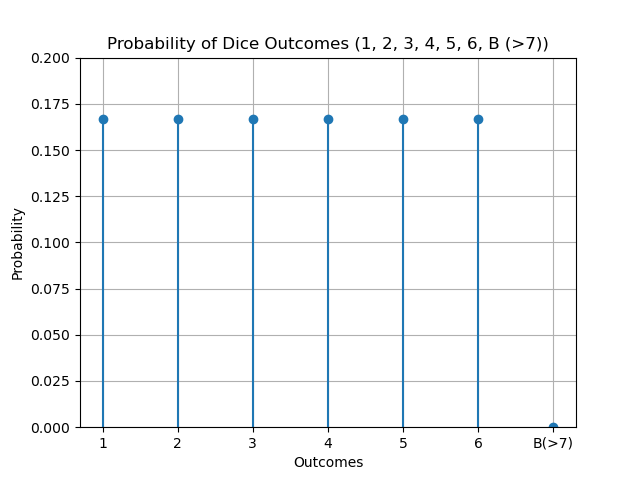
\includegraphics[width=\columnwidth]{figs/fig.png}
    \caption{Probability analysis of dice roll events}
    \label{fig:event_probs}
\end{figure}

\end{document}

